%---------------------
\pagestyle{plain}
\setcounter{page}{1}
\pagenumbering{arabic}
%---------------------

\chapter{برخی مفاهیم اولیه}
در این فصل سعی شده خواننده با مفاهیم مقدماتی کار آشنا شود. بعضی از مفاهیم ممکن است مستقیما در ادامه استفاده شده باشند و بعضی دیگر ممکن است مستقیما در ادامه وارد بحث نشده باشند اما آشنایی با آن‌ها برای درک بهتر واجب است.
\section{نظریه تعبیر مجرد}

در این بخش مفاهیم اولیه‌ی نظریه تعبیر مجرد را معرفی می‌کنیم.\\

\begin{defn}
	(ترتیب جزئی):
	اگر 
	$\mathbf{P}$
	یک مجموعه باشد و 
	$\mathbb{\leq}$
	یک رابطه روی این مجموعه باشد به‌طوریکه:
	$$
	1.\forall \mathbf{a} \in \mathbf{P}: \mathbf{a\leq a}$$
	$$2.\forall \mathbf{a,b} \in \mathbf{P}: (\mathbf{a \leq b \land b \leq a}) \rightarrow
	\mathbf{a=b} $$ 
	$$3.\forall \mathbf{a,b,c} \in \mathbf{P}: a \leq b \land b \leq c \rightarrow a \leq c$$
	آنگاه به زوج 
	$(\mathbf{P},\leq)$
	یک ترتیب جزئی می‌گوییم.
	
\end{defn}

در ادامه خواهیم دید که معنای برنامه‌های کامپیوتری که به یک زبان برنامه نویسی نوشته می‌شوند را می‌شود به شکل یک ترتیب جزئی دید. ترتیب‌های جزئي به عنوان یک نظریه ریاضی مطالعه شده‌اند و اگر معناشناسی یک برنامه را بتوانیم به این شکل بیان کنیم می‌توانیم از خصوصیاتی که در مورد ترتیب جزئی می‌دانیم در جهت کار با معناشناسی استفاده کنیم. 

\begin{defn}
	(اتصال گالو):
	اگر 
	$(\mathbf{C},\sqsubseteq)$
	و
	$(\mathbf{A},\preceq)$
	دو ترتیب جزئی باشند و دو تابع \\
	$\alpha : \mathbf{C \rightarrow A}$
	و
	$\gamma : \mathbf{A \rightarrow C}$
	را داشته باشیم که:
	$$
	\forall \mathbf{c \in C}: \forall \mathbf{a \in A}: 
	\alpha(\mathbf{c}) \preceq \mathbf{a} \leftrightarrow 
	\mathbf{c} \sqsubseteq \gamma(\mathbf{a})
	$$
\end{defn}


\section{روش وارسی مدل}

روش وارسی مدل یک روش صوری است که برای درستی‌یابی سیستم‌های مختلف استفاده می‌شود. در این روش معمولا ابتدا یک ماشین حالات متناهی از روی سیستم مورد بررسی ساخته می‌شود، سپس بررسی‌هایی که قرار است روی سیستم اصلی انجام شوند، روی این ماشین( مدل) انجام می‌شود. در بررسی صحت کارکرد برنامه‌های کامپیوتری از این روش استفاده می‌شود اما این تنها مورد استفاده از این روش نیست و هر منظومه‌ی دیگری که قابلیت بیان به صورت صوری را داشته باشد قابل بررسی با این روش هست. مثلا می‌توان از این روش برای بررسی صحت عملکرد برنامه‌ی قطارهای شهری استفاده کرد; در حالتی که مثلا خصوصیات مورد بررسی ما عدم رخ دادن تصادف بین قطارها یا پوشش تمام  مناطق شهر باشد. مثال های دیگر استفاده‌ی این روش در علوم کامپیوتر می تواند بررسی صحت عملکرد یک پردازنده یا مثلا الگوریتم تقسیمِ وظایف یک سیستم عامل باشد. این مثال‌ها هیچ یک برنامه‌ی کامپیوتری نیستند( هر چند که ممکن است مجبور باشیم از یک برنامه‌ی کامپیوتری برای پیاده سازی آن‌ها کمک بگیریم که در آن صورت بررسی صحت عملکرد آن برنامه‌ی کامپیوتری داستانی دیگر خواهد داشت) اما قابل بیان به صورت صوری به جای زبان طبیعی هستند.

ایده‌ی روش وارسی مدل از منطق‌های زمانی مختلف استفاده می‌کند. منطق زمانی یک نوع منطق موجهات است. منطق‌های موجهات از گسترش زبان منطق کلاسیک با اضافه کردن ادات وجهی گوناگون، با معانی متفاوتی که ممکن است در زبان طبیعی داشته باشند، ساخته می‌شوند. این ادوات غالبا در زبان طبیعی نقش قید را دارند. منطق‌های زمانی بخشی از منطق‌های موجهات هستند که به صوری‌گری ما مفهوم زمان را هم اضافه می‌کنند، یعنی قیدهایی مانند فعلا، بعدا و قبلا. منطقی که در اینجا بیان می‌کنیم \lr{LTL} نام دارد که یکی از منطق‌های زمانی است که برای روش وارسی مدل استفاده می‌شود.

ابتدا زبان این منطق را بیان می‌کنیم و سعی می‌کنیم به طور غیر دقیق در مورد معنای فرمول‌های این زبان به خواننده یک درک شهودی بدهیم; سپس به سراغ معناشناسی صوری این منطق می‌رویم.

\subsection{زبان \lr{LTL}}
\begin{defn}
	هر عضو مجموعه‌ی $\Phi$ یک فرمول در زبان \lr{LTL} است( و $\Pi$ مجموعه‌ی فرمول‌های اتمی است و $\pi \in \Pi$):
	$$
	\Pi \subset \Phi,
	$$
	$$
	\phi \in \Phi \Leftrightarrow
	\phi ::= \pi | \phi \land \phi | \phi \lor \phi |
	\neg \phi | \phi \rightarrow \phi  |
	\bigcirc \phi | \diamond \phi | \Box \phi |
	\phi \mathcal{U}\phi | \phi \mathcal{R}\phi | \phi \mathcal{W} \phi | \phi \mathcal{M} \phi
$$	
	
\end{defn}
اولین نکته‌ای که برای فرمول‌های این زبان به آن نیاز داریم این است که در این منطق ما زمان را با اعداد طبیعی و هر خاصیتی که در موردشان تعریف شده نشان می‌دهیم. یعنی برای یک فرمول، زمان از عدد ۰ شروع شده و تا ابد ادامه خواهد داشت و حین گذر زمان ممکن است ارزش فرمول‌ها تغییر کند. مسلما پس از بررسی معناشناسی صوری بهتر می‌شود این مفهوم را به طور شهودی حس کرد، اما به هر حال به خواننده پیشنهاد می‌شود پیش از رسیدن به آن بخش به ادامه‌ی این بخش هم توجه شود. 

در این زبان ادوات کلاسیک 
$\neg, \rightarrow, \land, \lor$
هستند با همان معنایی که در منطق گزاره‌ای کلاسیک داشتند.
در ادوات جدید 
$\bigcirc \phi$
به معنای برقرار بودن این فرمول دقیقا در لحظه‌ی بعدی( دقیقا یک لحظه) است، مثلا در شکل زیر با در نظر گرفتن اینکه در زمان 0 هستیم، این فرمول در لحظه‌ی ۱ برقرار است.
	\begin{center}
	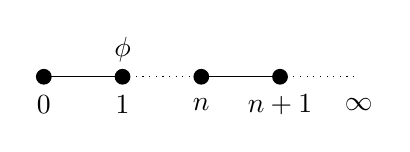
\begin{tikzpicture}
	\node at (1,0.35) (phi) {$\phi$};
	\node at (1,-0.35) (1) {$1$};
	\node at (0,-0.35) (0) {$0$};
	\node at (2,-0.35) (n) {$n$};
	\node at (3,-0.35) (1) {$n+1$};
	\node at (4,-0.35) (1) {$\infty$};
	\fill (0,0) circle (0.1cm);
	\fill (1,0) circle (0.1cm);
	\fill (2,0) circle (0.1cm);
	\fill (3,0) circle (0.1cm);
	\path (0,0) edge (1,0) 
	(1,0) edge[dotted] (2,0)
	(2,0) edge (3,0)
	(3,0) edge[dotted] (4,0);
	\end{tikzpicture}
\end{center}
$\diamond \phi$
به معنای برقرار بودن این فرمول در یک لحظه‌ای در آینده است( که الزاما لحظه‌ی بعدی نیست، مثلا لحظه‌ی $n$ام).
\begin{center}
	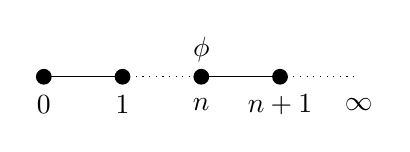
\begin{tikzpicture}
	\node at (2,0.35) (phi) {$\phi$};
	\node at (1,-0.35) (1) {$1$};
	\node at (0,-0.35) (0) {$0$};
	\node at (2,-0.35) (n) {$n$};
	\node at (3,-0.35) (1) {$n+1$};
	\node at (4,-0.35) (1) {$\infty$};
	\fill (0,0) circle (0.1cm);
	\fill (1,0) circle (0.1cm);
	\fill (2,0) circle (0.1cm);
	\fill (3,0) circle (0.1cm);
	\path (0,0) edge (1,0) 
	(1,0) edge[dotted] (2,0)
	(2,0) edge (3,0)
	(3,0) edge[dotted] (4,0);
	\end{tikzpicture}
\end{center}


$\Box \phi$
به معنای برقرار بودن این فرمول در همه‌ی لحظات آینده است که دوگان ادات قبلی است( با این فرض که در زمان ۰ هستیم و این حرف زده شده).
\begin{center}
	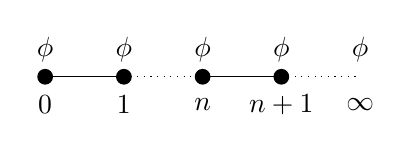
\begin{tikzpicture}
	\node at (1,0.35) (phi) {$\phi$};
	\node at (0,0.35) (phi) {$\phi$};
	\node at (2,0.35) (phi) {$\phi$};
	\node at (3,0.35) (phi) {$\phi$};
	\node at (4,0.35) (phi) {$\phi$};
	\node at (4,-0.35) (1) {$\infty$};
	\node at (1,-0.35) (1) {$1$};
	\node at (0,-0.35) (0) {$0$};
	\node at (2,-0.35) (n) {$n$};
	\node at (3,-0.35) (1) {$n+1$};
	
	\fill (0,0) circle (0.1cm);
	\fill (1,0) circle (0.1cm);
	\fill (2,0) circle (0.1cm);
	\fill (3,0) circle (0.1cm);
	\path (0,0) edge (1,0) 
	(1,0) edge[dotted] (2,0)
	(2,0) edge (3,0)
	(3,0) edge[dotted] (4,0);
	\end{tikzpicture}
\end{center}
$\phi \mathcal{U}\psi$
به این معنی است که فرمول سمت چپی حداقل تا قبل از اینکه فرمول سمت راستی برقرار شود، برقرار است.( مثلا اگر بگوییم "تا وقتی که باران نباریده زمین خشک است" در این صورت "زمین خشک است" به جای فرمول سمت چپ و "باران باریده است" فرمول سمت راست است).
\begin{center}
	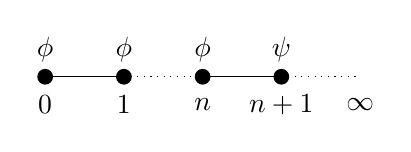
\begin{tikzpicture}
	\node at (1,0.35) (phi) {$\phi$};
	\node at (0,0.35) (phi) {$\phi$};
	\node at (2,0.35) (phi) {$\phi$};
	\node at (3,0.35) (phi) {$\psi$};
	\node at (1,-0.35) (1) {$1$};
	\node at (0,-0.35) (0) {$0$};
	\node at (2,-0.35) (n) {$n$};
	\node at (3,-0.35) (1) {$n+1$};
	\node at (4,-0.35) (1) {$\infty$};
	\fill (0,0) circle (0.1cm);
	\fill (1,0) circle (0.1cm);
	\fill (2,0) circle (0.1cm);
	\fill (3,0) circle (0.1cm);
	\path (0,0) edge (1,0) 
	(1,0) edge[dotted] (2,0)
	(2,0) edge (3,0)
	(3,0) edge[dotted] (4,0);
	\end{tikzpicture}
\end{center}


$\phi \mathcal{R}\psi$
که دوگان ادات قبلی است، به این معنی است که اگر خبر از وجود زمانی داشته باشیم که در آن فرمول سمت چپی برقرار باشد، تا آن لحظه و در خود آن لحظه فرمول سمت راستی برقرار است و اگر چنین لحظه‌ای وجود نداشته باشد، فرمول سمت راستی همیشه برقرار خواهد بود.
\begin{center}
	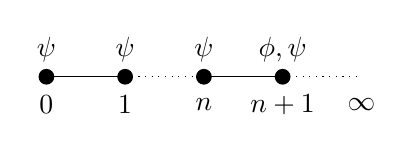
\begin{tikzpicture}
	\node at (1,0.35) (psi) {$\psi$};
	\node at (0,0.35) (psi) {$\psi$};
	\node at (2,0.35) (psi) {$\psi$};
	\node at (3,0.35) (psi) {$\phi,\psi$};
	\node at (1,-0.35) (1) {$1$};
	\node at (0,-0.35) (0) {$0$};
	\node at (2,-0.35) (n) {$n$};
	\node at (3,-0.35) (1) {$n+1$};
	\node at (4,-0.35) (1) {$\infty$};
	\fill (0,0) circle (0.1cm);
	\fill (1,0) circle (0.1cm);
	\fill (2,0) circle (0.1cm);
	\fill (3,0) circle (0.1cm);
	\path (0,0) edge (1,0) 
	(1,0) edge[dotted] (2,0)
	(2,0) edge (3,0)
	(3,0) edge[dotted] (4,0);
	\end{tikzpicture}
\end{center}

\begin{center}
	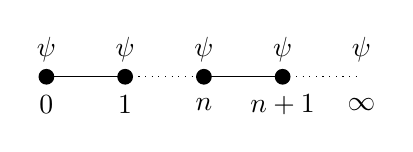
\begin{tikzpicture}
	\node at (1,0.35) (psi) {$\psi$};
	\node at (0,0.35) (psi) {$\psi$};
	\node at (2,0.35) (psi) {$\psi$};
	\node at (3,0.35) (psi) {$\psi$};
	\node at (4,0.35) (psi) {$\psi$};
	\node at (1,-0.35) (1) {$1$};
	\node at (0,-0.35) (0) {$0$};
	\node at (2,-0.35) (n) {$n$};
	\node at (3,-0.35) (1) {$n+1$};
	\node at (4,-0.35) (1) {$\infty$};
	\fill (0,0) circle (0.1cm);
	\fill (1,0) circle (0.1cm);
	\fill (2,0) circle (0.1cm);
	\fill (3,0) circle (0.1cm);
	\path (0,0) edge (1,0) 
	(1,0) edge[dotted] (2,0)
	(2,0) edge (3,0)
	(3,0) edge[dotted] (4,0);
	\end{tikzpicture}
\end{center}

$\phi \mathcal{W} \psi$
که حالت ضعیف‌تر 
$\mathcal{U}$ 
است به این معنی است که فرمول سمت چپی حداقل تا قبل از اینکه فرمول سمت راستی برقرار شود،  برقرار است و اگر خبر از زمانی نداشته باشیم که در آن فرمول سمت راستی برقرار باشد، فرمول سمت چپی تا ابد برقرار خواهد ماند.
\begin{center}
	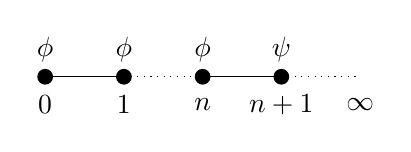
\begin{tikzpicture}
	\node at (1,0.35) (psi) {$\phi$};
	\node at (0,0.35) (psi) {$\phi$};
	\node at (2,0.35) (psi) {$\phi$};
	\node at (3,0.35) (psi) {$\psi$};
	\node at (1,-0.35) (1) {$1$};
	\node at (0,-0.35) (0) {$0$};
	\node at (2,-0.35) (n) {$n$};
	\node at (3,-0.35) (1) {$n+1$};
	\node at (4,-0.35) (1) {$\infty$};
	\fill (0,0) circle (0.1cm);
	\fill (1,0) circle (0.1cm);
	\fill (2,0) circle (0.1cm);
	\fill (3,0) circle (0.1cm);
	\path (0,0) edge (1,0) 
	(1,0) edge[dotted] (2,0)
	(2,0) edge (3,0)
	(3,0) edge[dotted] (4,0);
	\end{tikzpicture}
\end{center}

\begin{center}
	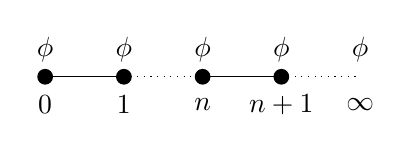
\begin{tikzpicture}
	\node at (1,0.35) (psi) {$\phi$};
	\node at (0,0.35) (psi) {$\phi$};
	\node at (2,0.35) (psi) {$\phi$};
	\node at (3,0.35) (psi) {$\phi$};
	\node at (4,0.35) (psi) {$\phi$};
	\node at (1,-0.35) (1) {$1$};
	\node at (0,-0.35) (0) {$0$};
	\node at (2,-0.35) (n) {$n$};
	\node at (3,-0.35) (1) {$n+1$};
	\node at (4,-0.35) (1) {$\infty$};
	\fill (0,0) circle (0.1cm);
	\fill (1,0) circle (0.1cm);
	\fill (2,0) circle (0.1cm);
	\fill (3,0) circle (0.1cm);
	\path (0,0) edge (1,0) 
	(1,0) edge[dotted] (2,0)
	(2,0) edge (3,0)
	(3,0) edge[dotted] (4,0);
	\end{tikzpicture}
\end{center}





$\phi \mathcal{M} \psi$
نیز دوگان ادات قبلی است و به این معنی است که تا قبل از اولین لحظه‌ای که در آن فرمول سمت چپ برقرار شده، به همراه همان لحظه، فرمول سمت راست برقرار است.

\begin{center}
	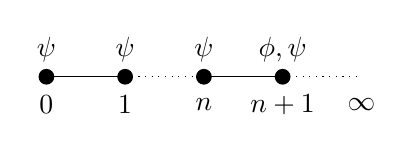
\begin{tikzpicture}
	\node at (1,0.35) (psi) {$\psi$};
	\node at (0,0.35) (psi) {$\psi$};
	\node at (2,0.35) (psi) {$\psi$};
	\node at (3,0.35) (psi) {$\phi,\psi$};
	\node at (1,-0.35) (1) {$1$};
	\node at (0,-0.35) (0) {$0$};
	\node at (2,-0.35) (n) {$n$};
	\node at (3,-0.35) (1) {$n+1$};
	\node at (4,-0.35) (1) {$\infty$};
	\fill (0,0) circle (0.1cm);
	\fill (1,0) circle (0.1cm);
	\fill (2,0) circle (0.1cm);
	\fill (3,0) circle (0.1cm);
	\path (0,0) edge (1,0) 
	(1,0) edge[dotted] (2,0)
	(2,0) edge (3,0)
	(3,0) edge[dotted] (4,0);
	\end{tikzpicture}
\end{center}


حال که به درکی شهودی از معنای فرمول‌های این زبان رسیده‌ایم، به بیان صوری این مفاهیم می‌پردازیم.

\subsection{معناشناسی \lr{LTL}}

معناشناسی صوری این منطق با استفاده از مدل‌های چهار مولفه‌ای 
$M=\langle S , T , V , I  \rangle$
تعریف می‌شود. در این سه مولفه، به مولفه اول یعنی $S$ مجموعه‌ی لحظه‌ها( یا جهان‌ها) می‌گوییم، ‌$T$ یک رابطه است روی $S$ که قالب مدل ما را مشخص می‌کند و $V$ یک تابع است که در هر لحظه ارزش گزاره‌های اتمی را مشخص می‌کند که با کمک آن می‌شود ارزش هر گزاره را در هر لحظه تعیین کرد و در نهایت $I$ نیز یک عضو از $S$ است که به عنوان لحظه‌ی ابتدایی مدل (که زمان در آن برابر ۰ است) در نظر گرفته می‌شود.

